\documentclass[9pt]{beamer}

\beamertemplatenavigationsymbolsempty
\renewcommand\mathfamilydefault{cmr}

\usepackage{xcolor}
\usepackage{pajmath}
\usepackage{booktabs}
\usepackage{colortbl}
\usepackage{tikz}
\usetikzlibrary{calc}
\usetikzlibrary{intersections}
\usetikzlibrary{datavisualization}
\usetikzlibrary{datavisualization.formats.functions}


\newcommand\VW{\V{W}}
\newcommand\bsigma{\boldsymbol{\sigma}}


\title{Neural Networks: Perceptrons}
\author{BIOE 498/598 PJ}
\date{Spring 2021}

\begin{document}

\maketitle

\begin{frame}{The artificial neuron}

A neuron connects a series on inputs (dendrites) to an output (axon).

\begin{center}
	output: $y$
	\raisebox{-0.2in}{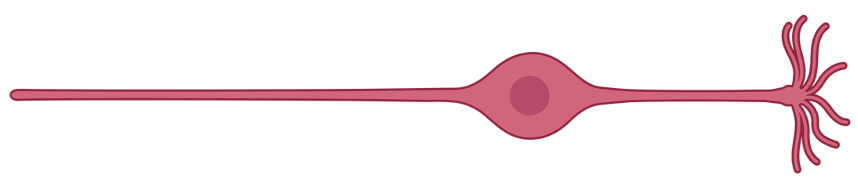
\includegraphics[width=0.5\textwidth]{figures/neuron}}
	$\left. \begin{matrix}x_1\\x_2\\ \vdots\\ x_n\end{matrix} \right\rbrace$ inputs
\end{center}
\pause
Our model needs to include two processes:
\begin{enumerate}
	\item The cell body (soma) combines all of the $n$ inputs.
	\item If the combined input exceeds a threshold, the output fires.
\end{enumerate}

\end{frame}

\begin{frame}{Modeling the artificial neuron}

\begin{center}
	output: $y$
	\raisebox{-0.2in}{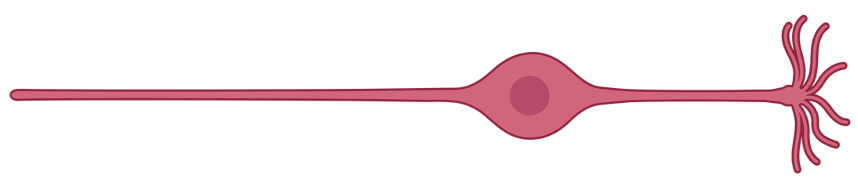
\includegraphics[width=0.5\textwidth]{figures/neuron}}
	$\left. \begin{matrix}x_1\\x_2\\ \vdots\\ x_n\end{matrix} \right\rbrace$ inputs
\end{center}
\bigskip
Let's model the combined input $z$ as a linear combination of the inputs.
\[ z = w_1x_1 + w_2x_2 + \cdots + w_nx_n = \V{w}\cdot\Vx \]

\pause
\bigskip
For now, let's assume the neuron ``fires'' based on the sign of $z$:
\[ y = \begin{cases} +1, & \V{w}\cdot\Vx > 0 \\ -1, & \V{w}\cdot\Vx < 0 \end{cases} \]

\end{frame}


\begin{frame}{Wait, what happened to the intercept?}

Our perceptron fires using the rule
\[ y = \begin{cases} +1, & \V{w}\cdot\Vx > 0 \\ -1, & \V{w}\cdot\Vx < 0 \end{cases} \]
Does this mean the perceptron hyperplane always passes through the origin?

\bigskip
\pause
\textbf{No.} We use a common ML trick to move the \emph{bias} (intercept) into the weight vector and expand \Vx\ with a dummy dimension containing 1.
\[ \V{w}\cdot\Vx = b \Leftrightarrow \vecthree{w_1}{w_2}{-b}\cdot\vecthree{x_1}{x_2}{1} = 0 \]

	
\end{frame}

\begin{frame}{Summary (so far)}

\begin{itemize}
	\item A perceptron is a simplistic model of a single neuron.
	\item A perceptron can learn to perform simple classification tasks using an update rule.
	\item<2-> \textbf{Imagine what a network of millions of perceptrons can learn!}
\end{itemize}
	
\end{frame}

\begin{frame}{Any nonlinearity will do}

Any nonlinear function can be an activation function.

\begin{columns}[T]
\begin{column}{0.3\textwidth}
	\begin{center}
		\textbf{Sign/step activation}
	\end{center}
\end{column}	
\begin{column}{0.3\textwidth}<2->
	\begin{center}
		\textbf{Sigmoid activation}
	\end{center}
\end{column}	
\begin{column}{0.3\textwidth}<3->
	\begin{center}
		\textbf{Rectified linear unit activation}
	\end{center}
\end{column}	
\end{columns}

\begin{columns}[T]
\begin{column}{0.3\textwidth}
	\begin{center}
		\[ \mathrm{sgn}(z) = \begin{cases} +1, & z > 0 \\ -1, & z < 0 \end{cases} \]
	\end{center}
\end{column}	
\begin{column}{0.3\textwidth}<2->
	\begin{center}
		\[ \sigma(z) = \frac{1}{1 + e^{-z}} \]
	\end{center}
\end{column}	
\begin{column}{0.3\textwidth}<3->
	\begin{center}
		\[ \mathrm{ReLU}(z) = \begin{cases} z, & z \ge 0 \\ 0, & z < 0 \end{cases} \]
	\end{center}
\end{column}	
\end{columns}


\begin{columns}[T]
\begin{column}{0.3\textwidth}
	\begin{center}
		\begin{tikzpicture}
			\draw [help lines,->] (-1,0) -- (1,0) node [below] {$z$};
			\draw [help lines,->] (0,-1) -- (0,1) node [left] {$y$};
			\draw [thick,blue] (-1,-1) node [left] {$-1$} -- (0,-1) (0,1) -- (1,1) node [right] {$+1$};
		\end{tikzpicture}
	\end{center}
\end{column}

\pause
\begin{column}{0.3\textwidth}<2->
	\begin{center}
		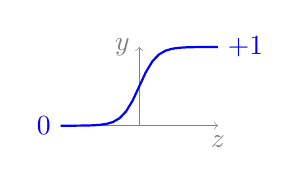
\begin{tikzpicture}
			\draw [help lines,->] (-1,0) -- (1,0) node [below] {$z$};
			\draw [help lines,->] (0,0) -- (0,1) node [left] {$y$};
			\draw [thick,blue, xscale=0.111, domain=-9:9] plot (\x, {1/(1+exp(-\x)});
			\node [blue,left] at (-1,0) {$0$};
			\node [blue,right] at (1,1) {$+1$};
		\end{tikzpicture}
	\end{center}
\end{column}

\pause
\begin{column}{0.3\textwidth}<3->
	\begin{center}
		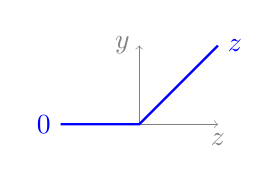
\begin{tikzpicture}
			\draw [help lines,->] (-1,0) -- (1,0) node [below] {$z$};
			\draw [help lines,->] (0,0) -- (0,1) node [left] {$y$};
			\draw [thick,blue] (-1,0) -- (0,0) -- (1,1);
			\node [blue,left] at (-1,0) {$0$};
			\node [blue,right] at (1,1) {$z$};
		\end{tikzpicture}
	\end{center}
\end{column}

\end{columns}	
\end{frame}


\begin{frame}{Multi-neuron (wide) perceptrons}

Neural networks use multiple neurons to learn different features from the \textbf{same inputs}.

\begin{center}
	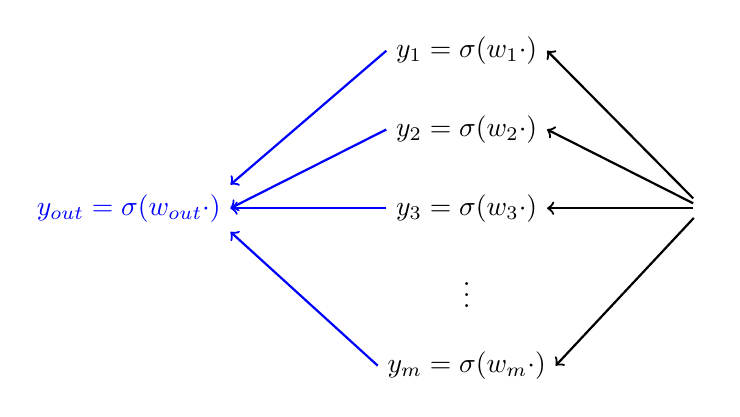
\begin{tikzpicture}
		\node (a) at (0,3) {$y_1 = \sigma(\V{w}_1\cdot\Vx)$};
		\node (b) at (0,2) {$y_2 = \sigma(\V{w}_2\cdot\Vx)$};
		\node (c) at (0,1) {$y_3 = \sigma(\V{w}_3\cdot\Vx)$};
		\node (d) at (0,0) {$\vdots$};
		\node (e) at (0,-1) {$y_m = \sigma(\V{w}_m\cdot\Vx)$};
		\node (s) at (3,1) {$\Vx$};
		\draw [->,thick] (s) -- (a.east);
		\draw [->,thick] (s) -- (b.east);
		\draw [->,thick] (s) -- (c.east);
		\draw [->,thick] (s) -- (e.east);
		\onslide<2->{
			\node [blue,left] (o) at (-3,1) {$y_\text{out} = \sigma(\V{w}_\text{out}\cdot\Vy)$};
			\draw [->,blue,thick] (a.west) -- (o.north east);
			\draw [->,blue,thick] (b.west) -- (o.east);
			\draw [->,blue,thick] (c.west) -- (o.east);
			\draw [->,blue,thick] (e.west) -- (o.south east);
		};
	\end{tikzpicture}
\end{center}

\onslide<2->{
	The outputs of each neuron are collected into a single neuron to predict the final class.
}

\end{frame}

\begin{frame}{A matrix formalism for perceptrons}

Consider a stack of $m$ neurons that are all connected to the same input~\Vx.
\begin{align*}
	z_1 &= \V{w}_1\cdot\Vx \\
	z_2 &= \V{w}_2\cdot\Vx \\
	 &\vdots \\
	z_m &= \V{w}_m\cdot\Vx \\
\end{align*}

\pause
The stack can be written as the product of the input~\Vx\ and a weight matrix
\[ \Vz = \V{W}\Vx \]
where each row in $\V{W}$ contins the weights for a single neuron
\[ \V{W} = \begin{pmatrix} \leftarrow \V{w}_1 \rightarrow \\
 						   \leftarrow \V{w}_2 \rightarrow \\
 						    \vdots \\
 						   \leftarrow \V{w}_m \rightarrow \\	
 \end{pmatrix}. \]
	
\end{frame}

\begin{frame}{Elementwise activation functions}

Let's define an \emph{elementwise} sigmoid activation function
\[ \bsigma(\Vz) = \begin{pmatrix} \sigma(z_1) \\ \sigma(z_2) \\ \vdots \\\sigma(z_n) \end{pmatrix}. \]
	
\pause
A stack of $m$ neurons can be written as
\begin{align*}
	\Vz &= \V{W}\Vx \\
	\Vy &= \bsigma(\Vz)	
\end{align*}
\pause
or, more succinctly as
\[ \Vy = \bsigma(\V{W}\Vx) \]
\pause
where
\[ \dim(\Vy)=m\times 1,\quad \dim(\Vz)=m\times 1 \]
\[ \dim(\V{W})=m\times n,\quad \dim(\Vx)=n\times 1 \]
\end{frame}

\begin{frame}{Completing our matrix formalism}
\begin{center}
	\small
	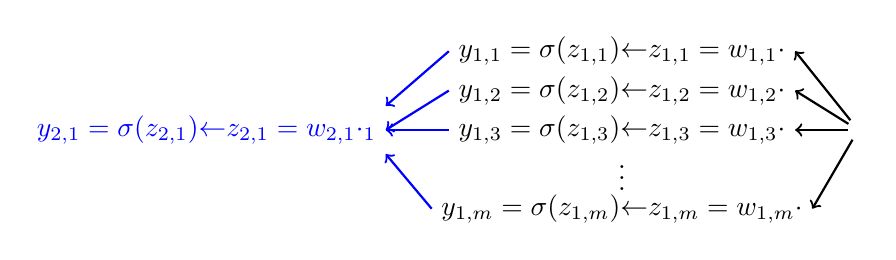
\begin{tikzpicture}
		\node (a) at (0,1.5) {$y_{1,1} =\sigma(z_{1,1}) \boldsymbol{\leftarrow} z_{1,1} = \V{w}_{1,1}\cdot\Vx$};
		\node (b) at (0,1) {$y_{1,2} =\sigma(z_{1,2}) \boldsymbol{\leftarrow} z_{1,2} = \V{w}_{1,2}\cdot\Vx$};
		\node (c) at (0,0.5) {$y_{1,3} =\sigma(z_{1,3}) \boldsymbol{\leftarrow} z_{1,3} = \V{w}_{1,3}\cdot\Vx$};
		\node (d) at (0,0) {$\vdots$};
		\node (e) at (0,-0.5) {$y_{1,m} =\sigma(z_{1,m}) \boldsymbol{\leftarrow} z_{1,m} = \V{w}_{1,m}\cdot\Vx$};
		\node (s) at (3,0.5) {$\Vx$};
		\draw [->,thick] (s) -- (a.east);
		\draw [->,thick] (s) -- (b.east);
		\draw [->,thick] (s) -- (c.east);
		\draw [->,thick] (s) -- (e.east);
		\node [blue,left] (o) at (-3,0.5) {$y_{2,1} =\sigma(z_{2,1}) \boldsymbol{\leftarrow} z_{2,1} = \V{w}_{2,1}\cdot\Vy_1$};
		\draw [->,blue,thick] (a.west) -- (o.north east);
		\draw [->,blue,thick] (b.west) -- (o.east);
		\draw [->,blue,thick] (c.west) -- (o.east);
		\draw [->,blue,thick] (e.west) -- (o.south east);
	\end{tikzpicture}
\end{center}

\pause
\[  \Vy_2 = \bsigma(\Vz_2) \quad\leftarrow\quad
	\Vz_2 = \V{W}_2\Vy_1 \quad\leftarrow\quad
	\Vy_1 = \bsigma(\Vz_1) \quad\leftarrow\quad
	\Vz_1 = \V{W}_1\Vx	 \]

\pause
\[ \Vy_2 = \bsigma(\V{W}_2(\bsigma(\V{W}_1\Vx))) \]

\pause
\bigskip
In general, a network with $d$ layers is
\[ \Vy_d = \bsigma(\V{W}_d(\bsigma(\V{W}_{d-1}(\cdots\bsigma(\V{W}_2(\bsigma(\V{W}_1\Vx))))))). \]

\end{frame}

\begin{frame}{Deep learning with neural networks}

\[ \Vy_d = \bsigma(\V{W}_d(\bsigma(\V{W}_{d-1}(\cdots\bsigma(\V{W}_2(\bsigma(\V{W}_1\Vx))))))) \]

\bigskip
\begin{itemize}
	\item The number of neurons in each layer $i$ is the \emph{width} of the layer.
	\begin{itemize}
		\addtolength\itemsep{0.5\baselineskip}
		\item If the ($i-1$)th layer has $n$ outputs and the $i$th layer has $m$ outputs, the weight matrix $\V{W}_i$ has dimensions $m\times n$.
		\item The dimensions of the inputs \Vx\ and outputs $\Vy_d$ are fixed by the problem.
		\item Layer $1$ is called the \emph{input layer}, and layer $d$ is the \emph{output layer}.
		\item We can use as many nodes as we want in the \emph{hidden} layers.
	\end{itemize}
	\item<2-> The number of layers $d$ is the \emph{depth} of the neural network.
	\item<3-> \emph{Deep learning} means $d>2$.
\end{itemize}
	
\end{frame}

\begin{frame}{The importance of nonlinearity}

The nonlinear functions (like $\bsigma$) sandwiched between the layers are critical to deep learning.

\bigskip
Let's imagine what would happen if we removed them:
\begin{align*}
	\Vy_d &= \bsigma(\V{W}_d(\bsigma(\V{W}_{d-1}(\cdots\bsigma(\V{W}_2(\bsigma(\V{W}_1\Vx))))))) \\
		 &= \V{W}_d(\V{W}_{d-1}(\cdots\V{W}_2(\V{W}_1\Vx))) \\
		 &= \V{W}_d \V{W}_{d-1} \cdots \V{W}_2 \V{W}_1 \Vx \\
		 &= \widetilde{\V{W}}\Vx
\end{align*}

\pause
\bigskip
Without the activation functions, the entire neural network reduces to a single linear system!
	
\end{frame}

\begin{frame}{Why do we want deep networks?}

\begin{itemize}
	\item The \emph{Universal Approximation Theorem} states that given enough neurons, a 2-layer (input/output) perceptron can learn any reasonable function.
	\item Neural networks are therefore universal function approximators.
\end{itemize}

\pause
\begin{itemize}
	\item Unfortunately, the theorem does not tell us how many neurons we need to approximate a given function.
	\item For complicated functions, evidence suggests the number is enormous!
\end{itemize}

\pause
\begin{itemize}
	\item Our brains are very deep, so it's reasonable to believe that deep networks learn more efficiently than wide ones.
	\item In practice this is almost certainly true.
	\item Deep learning reduces the total number of neurons needed to learn a function since each of the $d$ layers needs fewer than $1/d$-times the number of neurons.
\end{itemize}
	
\end{frame}

\begin{frame}{Why do deeper networks learn better?}
We can understand deep networks using examples from \emph{feature engineering}.

\bigskip
Imagine you wanted to learn a Michaelis-Menten function.
\begin{columns}
\begin{column}{0.4\textwidth}<2->
	\begin{center}
	\textbf{Single Layer}
	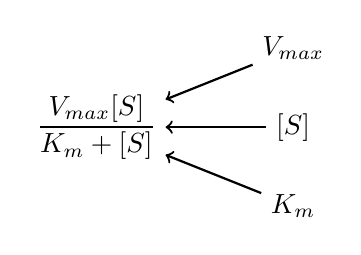
\begin{tikzpicture}[arr/.style={black,thick,->}]
		\node (Vmax) at (1,3) {$V_\text{max}$};
		\node (S) at (1,2) {$[S]$};
		\node (Km) at (1,1) {$K_m$};
		\node (full) at (-1.5,2) {$\displaystyle \frac{V_\text{max}[S]}{K_m+[S]}$};
		\draw [arr] (Vmax) -- (full);
		\draw [arr] (S) -- (full);
		\draw [arr] (Km) -- (full);
	\end{tikzpicture}	
\end{center}
\end{column}

\begin{column}{0.6\textwidth}<3->
	\begin{center}
	\textbf{Two Layers}
	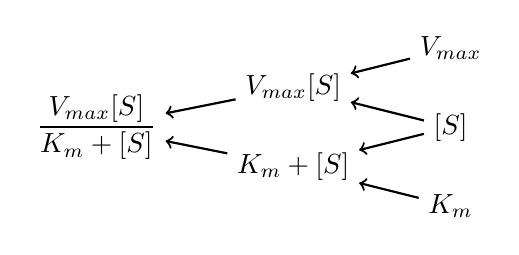
\begin{tikzpicture}[arr/.style={black,thick,->}]
		\node (Vmax) at (3,3) {$V_\text{max}$};
		\node (S) at (3,2) {$[S]$};
		\node (Km) at (3,1) {$K_m$};
		\node (VmaxS) at (1,2.5) {$V_\text{max}[S]$};
		\node (KmS) at (1,1.5) {$K_m + [S]$};
		\node (full) at (-1.5,2) {$\displaystyle \frac{V_\text{max}[S]}{K_m+[S]}$};
		\draw [arr] (Vmax) -- (VmaxS);
		\draw [arr] (S) -- (VmaxS);
		\draw [arr] (Km) -- (KmS);
		\draw [arr] (S) -- (KmS);
		\draw [arr] (VmaxS) -- (full);
		\draw [arr] (KmS) -- (full);
	\end{tikzpicture}	
\end{center}
\end{column}
	
\end{columns}

\bigskip
\onslide<4->{
	Each layer in the network only needs to improve the features for the next layer.
}

\end{frame}

\begin{frame}{Summary}

\begin{itemize}
	\addtolength\itemsep{0.5\baselineskip}
	\item Deep neural networks are built from layers in artificial neurons.
	\item Each neuron has the power of a linear classifier.
	\item Layers \textbf{must} be separated by nonlinear activation functions.
	\item Neural networks can learn nearly any function, but deep networks learn more efficiently.
	\item Each layer creates features for the subsequent layers to improve learning.
	\item<2-> \textbf{Next time:} Training a neural network to learn $Q$-factors.
\end{itemize}
	
\end{frame}

\end{document}
